\hypertarget{protocol_t_p_chart_color-p}{
\section{$<$ TPChartColor $>$ Protocol Reference}
\label{protocol_t_p_chart_color-p}\index{TPChartColor-p@{TPChartColor-p}}
}
{\tt \#import $<$TPParameterProtocols.h$>$}

Inheritance diagram for $<$ TPChartColor $>$::\begin{figure}[H]
\begin{center}
\leavevmode
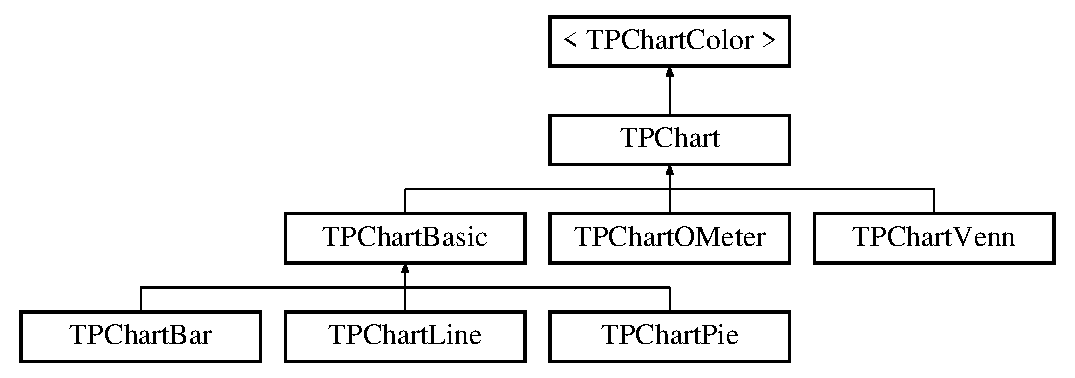
\includegraphics[height=4cm]{protocol_t_p_chart_color-p}
\end{center}
\end{figure}
\subsection*{Public Member Functions}
\begin{CompactItemize}
\item 
(void) - \hyperlink{protocol_t_p_chart_color-p_cce9d732cc3fd7f56a1e14fb73e8a1cb}{setChartColors:}
\end{CompactItemize}


\subsection{Detailed Description}
Protocol for charts who can have colors 

\subsection{Member Function Documentation}
\hypertarget{protocol_t_p_chart_color-p_cce9d732cc3fd7f56a1e14fb73e8a1cb}{
\index{TPChartColor-p@{TPChartColor-p}!setChartColors:@{setChartColors:}}
\index{setChartColors:@{setChartColors:}!TPChartColor-p@{TPChartColor-p}}
\subsubsection[{setChartColors:}]{\setlength{\rightskip}{0pt plus 5cm}- (void) setChartColors: ({\bf TPParameterChartColor} $\ast$) {\em colors}}}
\label{protocol_t_p_chart_color-p_cce9d732cc3fd7f56a1e14fb73e8a1cb}


Set color parameters \begin{Desc}
\item[Parameters:]
\begin{description}
\item[{\em colors}]colors to set \end{description}
\end{Desc}


The documentation for this protocol was generated from the following file:\begin{CompactItemize}
\item 
TPParameterProtocols.h\end{CompactItemize}
